\chapter{Project Management}

In this chapter, we will explain how we have planned this project and the tools we have used in order to achieve out objectives 
according to the time restrictions we have had. A good planning is essential in any project that seeks to meet its expectations.

\section{Development Frameworks and Methodologies}
We have followed the Scrum agile framework in this project, one of the most popular frameworks for implementing agile development.

As for the life cycle model, we have employed an iterative and incremental model, which is a method of software development that is 
modeled around a gradual increase in feature additions and a cyclical release and upgrade pattern.\cite{techopediaIterative}

Iterative and incremental software development begins with planning and habitually continues through iterative development cycles 
involving continuous user feedback and the incremental addition of features concluding with the deployment of completed software 
at the end of each cycle. 

\bigskip
\section{Planning}
In this project, we have used Redmine to mainly keep control of our tasks and their planning.

\begin{figure}
	\centering
	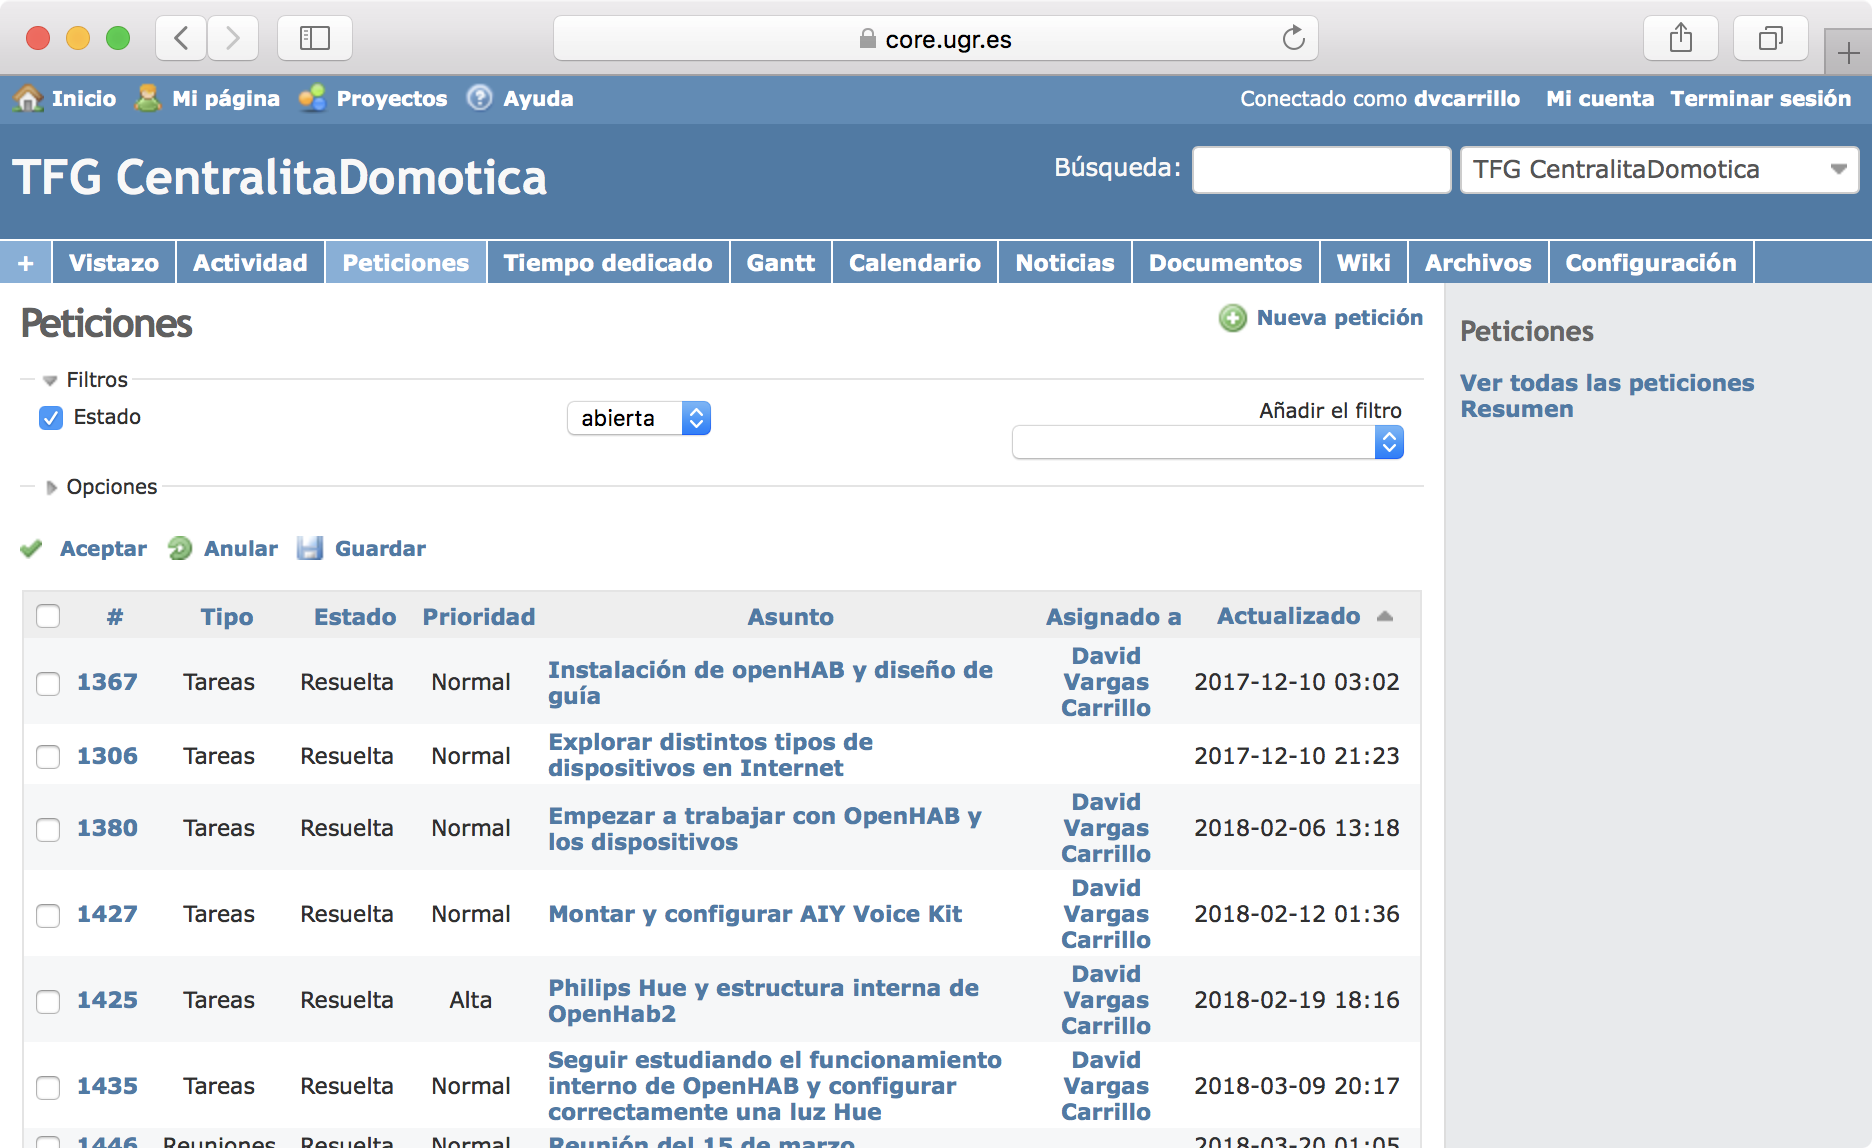
\includegraphics[width=1\textwidth]{images/Chapter_02/redmine.png}
	\caption{Redmine web application}
	\label{fig:redmine}
\end{figure}

Redmine is a free and open-source flexible project management web application. It features per project wikis and forums, time 
tracking, and flexible, role-based access control. It includes a calendar and Gantt charts to aid visual representation of projects 
and their deadlines. Redmine integrates with various version control systems and includes a repository browser and diff viewer.

The planning that we have followed for developing this project is divided in eight main tasks, specified below.
\begin{itemize}
	\item \textbf{First meetings and conception of the project}: we meet in a few sessions to determine the project and the 
	objectives to fulfill.
	\item \textbf{Exploration of domotic devices}: we explored suitable domotic devices that can be added to the home automation
	system.
	\item \textbf{Learning openHAB and working with domotic devices}: we learned the basics of this home automation system, installed
	it on different ways and tested different smart devices.
	\item \textbf{Building and configuring the AIY Voice Kit}: this task is about the installation and configuration of the Google 
	AIY Voice Kit in order to integrate it to our system.
	\item \textbf{Understanding the internal functioning of openHAB}: we studied and documented how openHAB works internally, from
	a developer perspective.
	\item \textbf{Designing and implementing the voice assistant}: in this task we designed the custom voice assistant, inside of 
	the AIY Voice Kit, and implemented it in Python.
	\item \textbf{Addition of extra functionalities}: we added automation, access from everywhere and management from a mobile 
	application.
	\item \textbf{Thesis writing}: this task contains everything related to the thesis writing in LaTeX.
\end{itemize}

A time distribution of these previous tasks can be seen in the Gantt diagram in figure \ref{fig:gantt}.

\begin{sidewaysfigure}
	\centering
	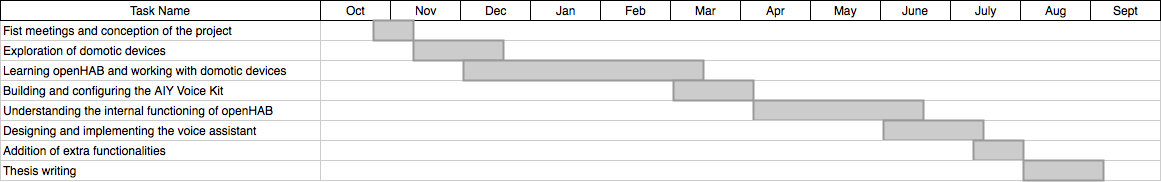
\includegraphics[width=1\textwidth]{images/Chapter_02/gantt.png}
	\caption{Gantt diagram of the tasks of this project}
	\label{fig:gantt}
\end{sidewaysfigure}

\bigskip
\section{Documentary Management}
In this project we maintained a repository where we uploaded all the changes related to this project. This repository is composed
by copies of the bibliography, partial documentation we wrote during the development of the project, source code files and the most
recent copy of all the files related to this thesis.

For version control, we used SVNManager, a PHP web-based tool to administer a Apache Subversion repository server. SmartSVN, on
our computers, scanned and committed the changes we made to these files.

\bigskip
\section{Estimated Total Cost}

The final cost of this project is specified in the table \ref{table:total-cost}. We have considered all the devices that can make
the final system work. The displayed approximate prices have been set according to the Spanish market. The cost of labour has been 
calculated on the basis of the price of EUR 40 per hour.

\begin{table}[]
	\centering
	\resizebox{\textwidth}{!}{%
		\begin{tabular}{|l|l|l|}
			\hline
			\multicolumn{1}{|c|}{\textbf{Product}} & \multicolumn{1}{c|}{\textbf{QTY}} & \multicolumn{1}{c|}{\textbf{Price}} \\ \hline
			Raspberry Pi 3 Model B+ & 1 piece & EUR 40 \\ \hline
			SanDisk microSDHC UHS-I 16GB & 1 piece & EUR 10 \\ \hline
			Google AIY Voice Kit & 1 piece & EUR 34 \\ \hline
			\begin{tabular}[c]{@{}l@{}}Philips Hue White and Color Ambiance Starter Kit\\ (Twin Pack Bulb with Bridge)\end{tabular} & 1 piece & EUR 90 \\ \hline
			Labour cost (EUR 40 per hour) & 150 hours & EUR 6,000 \\ \hline
			\multicolumn{2}{|l|}{\textbf{TOTAL}} & \textbf{EUR 6,174} \\ \hline
		\end{tabular}%
	}
	\caption{Estimated total cost of this project}
	\label{table:total-cost}
\end{table}

